\documentclass[aspectratio=169]{beamer}
\usepackage{beamerthemeAMU}
\usepackage{amsmath}
\usepackage{booktabs}
\usepackage{array}
\usepackage{listings}
\usepackage{hyperref}
\usepackage[T1]{fontenc}
\usepackage[utf8]{inputenc}

% Listing style for code snippets (kept consistent with prior weeks)
\lstset{basicstyle=\ttfamily\small,keywordstyle=\color{AMU_dk2}\bfseries,commentstyle=\itshape\color{gray},showstringspaces=false,columns=flexible}

\title{Large Language Models in Data Science}
\subtitle{Week 4: Text Classification — Intent Routing for AMU Chatbot}
\author{Sebastian Mueller}
\institute{Aix-Marseille Universit\'e}
\date{2025-2026}

\begin{document}

\begin{frame}[plain]
  \titlepage
\end{frame}

\begin{frame}{Session Overview}
  \begin{columns}[T,onlytextwidth]
    \begin{column}{0.55\linewidth}
      \textbf{Lecture (15min)}
      \begin{enumerate}
        \item Problem framing: intent classification
        \item Dataset design and labels
        \item Baselines: regex rules
        \item Embeddings + Logistic Regression
        \item Zero-shot NLI pipeline
        \item LLM prompting for classification
        \item Comparison and trade-offs
      \end{enumerate}
    \end{column}
    \begin{column}{0.4\linewidth}
      \textbf{Lab (2.5h)}
      \begin{itemize}
        \item Build 4 classifiers (regex, embed+LR, zero-shot, LLM)
        \item Measure accuracy and latency
        \item Analyze failure cases and label phrasing
        \item Extend training data and re-evaluate
        \item Optional: add a new intent
      \end{itemize}
    \end{column}
  \end{columns}
\end{frame}

\section{Project Context}
\begin{frame}{AMU Chatbot}
  \begin{center}
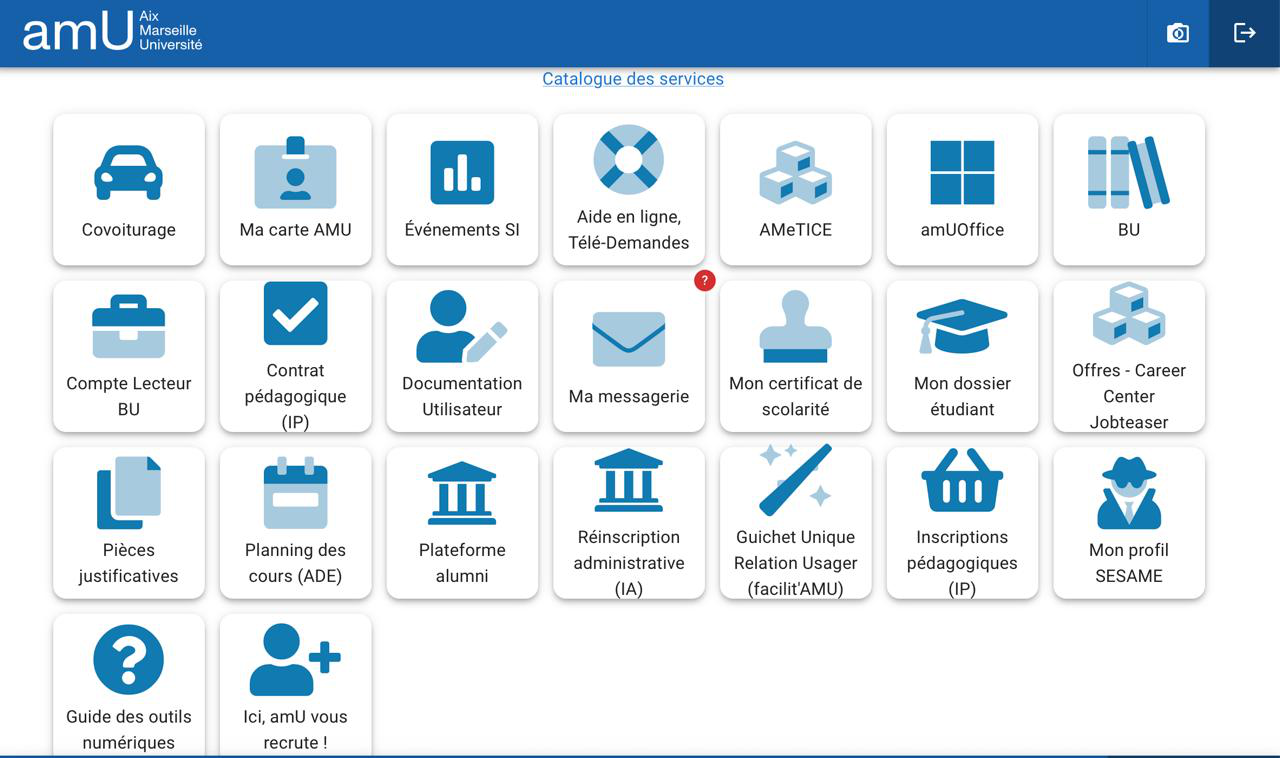
\includegraphics[width=0.5\linewidth]{ent_etudiant.png}
  \end{center}
  \begin{itemize}
    \item AMU is developing a student support chatbot (in French and English).
    \item The chatbot needs to route student queries to the right AMU service/tool.
    \item Reliable intent classification is critical for user satisfaction.
  \end{itemize}
\end{frame}



\begin{frame}{Project: AMU Chatbot Brain}
  \begin{itemize}
    \item \textbf{Goal}: Map student queries to AMU services (\emph{intent routing}).
    \item \textbf{Task}: Given a short query, predict one of 5 intents.
    \item \textbf{Why it matters}: Enables reliable hand-off to the right tool/API.
  \end{itemize}
  \vspace{0.4em}
  \textbf{Intents (lab setup)}
  \begin{itemize}
    \item \texttt{get\_schedule} (Planning des cours / ADE)
    \item \texttt{check\_email} (Ma messagerie)
    \item \texttt{register\_classes} (Inscriptions p\'edagogiques / IP)
    \item \texttt{get\_student\_card} (Ma carte AMU)
    \item \texttt{find\_library\_info} (BU / Compte Lecteur BU)
  \end{itemize}
\end{frame}

\section{Methods}

\begin{frame}{Four Approaches at a Glance}
  \begin{itemize}
    \item \textbf{Regex baseline}: Fastest and transparent; brittle, hard to scale.
    \item \textbf{Embeddings + LogisticRegression}: High accuracy with small data; fast inference; retrain to add intents.
    \item \textbf{Zero-shot classification (MNLI)}: No training; label phrasing matters; moderate latency.
    \item \textbf{LLM prompt}: Most flexible and often strongest; slowest and requires parsing structured output.
  \end{itemize}
\end{frame}

\begin{frame}{Evaluation Plan}
  \begin{itemize}
    \item \textbf{Metrics}: \emph{Accuracy} (correct label) and \emph{Latency} (ms per query).
    \item \textbf{Protocol}: Run all methods on the same test set; record predictions+timings.
    \item \textbf{Compute note}: Latency varies by device (CPU vs. GPU); compare on same hardware when possible.
    \item \textbf{Reproducibility}: Pin model names/revisions; save prompts and candidates; fix seeds where relevant.
  \end{itemize}
\end{frame}

\begin{frame}{Design Tips}
  \begin{itemize}
    \item \textbf{Regex}: Prefer precise patterns; avoid overbroad keywords (e.g., plain "amu").
    \item \textbf{Embeddings}: Use multilingual sentence models; validate with cross-validation if data grows.
    \item \textbf{Zero-shot}: Use descriptive, possibly multilingual labels (\emph{emploi du temps} vs. \emph{get\_schedule}).
    \item \textbf{LLM prompting}: Specify role, label set, and \emph{strict output format} (JSON / one token).
  \end{itemize}
\end{frame}

\section{Takeaways}

\begin{frame}{Key Takeaways \& Recommendations}
  \begin{itemize}
    \item Start with \textbf{embeddings + LR} for a strong, fast baseline.
    \item Use \textbf{zero-shot} for quick prototyping or new intents without data.
    \item Keep a small \textbf{regex layer} for guardrails and trivial routes.
    \item Add an \textbf{LLM fallback} for ambiguous/edge cases; require structured outputs and log decisions.
  \end{itemize}
\end{frame}

\end{document}
